\documentclass{standalone}
\usepackage{tikz}

\begin{document}

	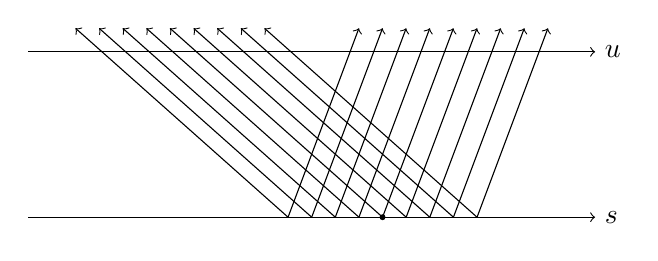
\begin{tikzpicture}[scale = 0.3, baseline]
	
		\draw[->] (-11, 0) -- (13, 0);
		\draw[->] (-11, 7) -- (13, 7);
		
		\node[right] at (13, 0) {$s$}; 
		\node[right] at (13, 7) {$u$}; 
		
		\draw[->] (0, 0) -- (-9, 8);
		\draw[->] (1, 0) -- (-8, 8);
		\draw[->] (2, 0) -- (-7, 8);
		\draw[->] (3, 0) -- (-6, 8);
		\draw[->] (4, 0) -- (-5, 8);
		\draw[->] (5, 0) -- (-4, 8);
		\draw[->] (6, 0) -- (-3, 8);
		\draw[->] (7, 0) -- (-2, 8);
		\draw[->] (8, 0) -- (-1, 8);
		
		\draw[->] (0, 0) -- (3, 8);
		\draw[->] (1, 0) -- (4, 8);
		\draw[->] (2, 0) -- (5, 8);
		\draw[->] (3, 0) -- (6, 8);
		\draw[->] (4, 0) -- (7, 8);
		\draw[->] (5, 0) -- (8, 8);
		\draw[->] (6, 0) -- (9, 8);
		\draw[->] (7, 0) -- (10, 8);
		\draw[->] (8, 0) -- (11, 8);
		
		\draw[fill] (4, 0) circle [radius = 0.1];
		
		%		\draw (0, 0) -- (0, {-sqrt(81/49 + 1)});
		%		\draw (0, 0) -- (9/7, -1);
		%		\draw (0, -1) arc (-90 : -90 + atan(9/7) : 1);
		%		
		%		\node[below right] at (0, 0) {$\theta$};
	\end{tikzpicture}

\end{document}